%! TEX program = xelatex
\documentclass{report}
% provides basic settings for ctex document
\usepackage[UTF8, heading=true]{ctex}
\usepackage{fancyhdr}
\usepackage{tocloft}
\usepackage[margin=1in]{geometry}
\usepackage{metalogo}                   % \XeLaTeX
\usepackage{float}                      % figure H flag
\usepackage{microtype}                  % break long words
\usepackage[hidelinks]{hyperref}
\usepackage{tabularx}
\usepackage{amsmath}
\usepackage{lmodern}                    % allow fonts to scale
\usepackage{placeins}
\usepackage{multirow}                   % multirow, multicolumn support
\usepackage{booktabs}                   % toprule, cmidrule support
\usepackage{caption}

% make chapter stay in the same page
%\makeatletter
%\renewcommand\chapter{\thispagestyle{plain}%
%\global\@topnum\z@
%\@afterindentfalse
%\secdef\@chapter\@schapter}
%\makeatother

\fancyhead{}
\renewcommand{\sectionmark}[1]{\markleft{#1}}
\renewcommand{\partmark}[1]{\markright{#1}}
\lhead{\leftmark}
\rhead{\rightmark}
% see $(texdoc ctex) for details
\ctexset{
    chapter = {
        format += \flushleft,
        number = \arabic{chapter},
    },
    section = {
        format += \flushleft,
    },
    appendix = {
        number = \Alph{chapter},
        name = {附录},
    },
}

\pagestyle{fancy}

%\setlength\cftaftertoctitleskip{2em}

% provides code input support
\usepackage{xparse}                     % newcommand multiple optional arguments
\usepackage{listings}                   % code
\usepackage{fontspec}
\usepackage{lmodern}

%\newfontfamily\codeF{Fira Code}

\setmonofont[
    Contextuals={Alternate},
    ItalicFont = Fira Code      % to avoid font warning
]{Fira Code}

% usage: \inputCode{[language] <path>}
% if language is not explicitly set, it's defaulted to c
\DeclareDocumentCommand{\inputCode}{ O{c} m }{
    {
        \lstinputlisting[
            basicstyle=\small\ttfamily,
            language={#1},
            tabsize=4,
            showstringspaces=false,
            breaklines=true,
            frame=shadowbox,
            framexleftmargin=10mm,
            rulesepcolor=\color{black},
            numbers=left,
            xleftmargin=4em,
        ]{#2}
    }
}

\DeclareDocumentCommand{\inputCodeSetLanguage}{ m }{
    \lstset{
        basicstyle=\small\ttfamily,
        language={#1},
        tabsize=4,
        showstringspaces=false,
        breaklines=true,
        frame=shadowbox,
        framexleftmargin=10mm,
        rulesepcolor=\color{black},
        numbers=left,
        xleftmargin=4em,
    }
}


\usepackage{xparse}
\usepackage{tcolorbox}
\usepackage{mdframed}

\tcbuselibrary{breakable}
\NewDocumentCommand{\exercise}{ m +m }{
    {
        \edef\originalParIndent{\the\parindent}
        \begin{tcolorbox}[breakable,arc=0mm,boxrule=0.4pt]
            \setlength{\parindent}{\originalParIndent}
            \noindent
            \textbf{\large Exercise #1}
            \indent
            #2
        \end{tcolorbox}
    }
}

% environment style of exercise, to feed special requirements
\NewDocumentEnvironment{exerciseEnv}{m}{
    \edef\originalParIndent{\the\parindent}
    \begin{tcolorbox}[breakable,arc=0mm,boxrule=0.4pt]
        \setlength{\parindent}{\originalParIndent}
        \noindent
        \textbf{\large Exercise #1}
        \indent
} {
    \end{tcolorbox}
}

\NewDocumentEnvironment{questionEnv}{}{
    \edef\originalParIndent{\the\parindent}
    \begin{tcolorbox}[breakable,arc=0mm,boxrule=0.4pt]
        \setlength{\parindent}{\originalParIndent}
        \noindent
        \textbf{\large Question}
        \indent
} {
    \end{tcolorbox}
}

% a raised rule
\NewDocumentCommand{\raisedrule}{ O{0em} m }{\leaders\hbox{\rule[#1]{1pt}{#2}}\hfill}

\NewDocumentEnvironment{exerciseSolution}{m}{
    {\noindent \textbf{\large Exercise #1 实验过程 \raisedrule[0.3em]{0.6pt}}}
} {
    \par
    {\noindent \textbf{\large \raisedrule[0.3em]{0.6pt} Exercise #1 实验过程}}
    \vspace{1em}
}

\NewDocumentEnvironment{answer}{}{
    {\noindent \textbf{\large Answer \raisedrule[0.3em]{0.6pt}}}
} {
    \par
    {\noindent \textbf{\large \raisedrule[0.3em]{0.6pt} Answer}}
    \vspace{1em}
}


% provides algorithm input support
\usepackage{algorithm}                  % algorithm pseudo code
\usepackage[noend]{algpseudocode}
\usepackage{caption}

% usage:
% \begin{simpleAlgorithm}{<algorithm-name>}
%     \Procedure{<procedure-name>}{$<parameters>$}
%     \State <statements>
%     \For{<condition>}
%     ...
%     \EndFor
%     \If{<condition>}
%         ...
%     \ElsIf{<condition>}
%         ...
%     \Else
%         ...
%     \EndIf
%     \State \Return <return val>
%     \EndProcedure
% \end{simpleAlgorithm}
%
% see $(texdoc algorithmic for details)
\NewDocumentEnvironment{simpleAlgorithm}{m}
{
\captionof{algorithm}{#1}
\hrule
\begin{algorithmic}[1]
} {
\end{algorithmic}
\hrule \vspace{1em}
}


%%%%%%%%%%%%%%%%%%%%%%%%%%%%%%%%
\graphicspath{{./res/}}

% report content %%%%%%%%%%%%
%%%%%%%%%%%%%%%%%%%%%%%%%%%%%
\begin{document}

% cover page
\begin{titlepage}
    \addtolength{\topmargin}{1cm}
    \centering
    
\includegraphics[width=0.6\textwidth]{hust.jpg}\par
    \vspace{0.5cm}
    {\Huge \heiti 操作系统课程设计报告}\par
    \vspace{10cm}
    {
        \large
        \begin{tabular}{r m{8em}}
            \makebox[6em][s]{学生姓名}:& 胡思勖 \\ \cline{2-2}
            %\makebox[6em][s]{学生姓名}:& 陈志浩 \\ \cline{2-2}
            %\makebox[6em][s]{学生姓名}:& 黄志强\\ \cline{2-2}
            \makebox[6em][s]{学号}:& U201514898\\ \cline{2-2}
            %\makebox[6em][s]{学号}:& U201514893\\ \cline{2-2}
            %\makebox[6em][s]{学号}:& U201514896\\ \cline{2-2}
            \makebox[6em][s]{专业}:& 计算机科学与技术\\ \cline{2-2}
            \makebox[6em][s]{班级}:& 计卓1501\\ \cline{2-2}
            \makebox[6em][s]{指导教师}:& 张杰 \\ \cline{2-2}
        \end{tabular}
    }
    \vfill
    2018-03-03
\end{titlepage}

\setcounter{tocdepth}{1}
\pagenumbering{Roman}
\tableofcontents

\newpage
\pagenumbering{arabic}
\setcounter{page}{1}



% chapter 1
\chapter{Booting a PC}
\label{cha:booting_a_pc}

\section{PC Bootstrap}
\par 这一部分主要介绍了x86语言以及PC的启动过程,并让我们熟悉了QEMU和GDB的调试方法。

\subsection{Getting Started with x86 assembly}
\par 通过阅读\emph{PC Assembly Language Book}\footnote{\url{https://pdos.csail.mit.edu/6.828/2017/readings/pcasm-book.pdf}}来学习x86的语法。注意这本书值使用的NASM汇编,但是实验中使用的是GNU的AT\&T语法。




% chapter 2
\chapter{基于pthread的形态学图像处理}
\section{实验目的与要求}
\begin{itemize}
    \item 掌握使用pthread的基本的并行编程设计方法以及调优方法;
    \item 掌握并行编程中基本的数据分块以及任务分解的方法。
    \item 使用pthread实现并行的形态学图像处理。
    \item 简要分析以及总结处理的结果。
\end{itemize}

\section{算法描述}
\par 使用多个线程对于一个图像进行蚀刻以及膨胀的算法如下,算法为一个线程的流程,而有多个这样的线程同时进行。
\begin{simpleAlgorithm}{pthread并行处理算法(一个线程)}
    \Procedure{PthreadParallel}{$blocks$}
    \While{true}
        \State lock\((blocks)\)
        \State get first block \(blk\) from \(blocks\)
        \If{\(blocks\).empty()}
            \State unlock\((blocks)\)
            \State \Return
        \EndIf
        \State unlock\((blocks)\)
        \State \Call{ErodeAndDilate}{$blk, kernel_e, kernel_d$}
    \EndWhile
    \EndProcedure
\end{simpleAlgorithm}
\par 算法中,\(blocks\)参数为一个工作队列,队列中的工作为原预处理过后的图片的子图片。在每个线程的每个循环中,首先锁住队列,从队列中获取一个子图片\(blk\)、解锁队列然后使用上一章中的ErodeAndDilate过程进行处理。如果\(blocks\)中没有子图片,说明处理完成,则此线程退出。
\par 主线程的流程如图\ref{fig:pthreadMain}所示。在进行预处理过后启动多个线程,然后等待所有线程竞争子图像、处理然后结束即可,最后保存处理的结果即可。
\begin{figure}[htpb]
    \centering
    
\includegraphics[width=0.95\linewidth]{pthreadMain.png}
    \caption{主线程流程}
    \label{fig:pthreadMain}
\end{figure}

\par 由于是使用pthread的并行算法,每一个线程处理一个部分,因此首先需要将数据分块(即分为算法中的\(blocks\))。分块方式如图\ref{fig:partition}所示。每块大小一样,在边缘部分如果块大小不符则按照原图的边缘进行裁减。因此,在进行处理时需要对于边缘部分进行考虑。
\begin{figure}[htpb]
    \centering
    
\includegraphics[width=0.76\linewidth]{partition.png}
    \caption{分块方法}
    \label{fig:partition}
\end{figure}

\section{实验方案}
\par 所有的开发与运行环境见附录\ref{cha:env},表\ref{tab:env},此后实验的开发与运行环境均相同,不再赘述。根据算法描述、分块方法以及主线程的流程编写程序并运行,然后观察结果并与串行的程序比较。经过多轮的比较以及参数调试后得出一个较好的效果。

\section{实验结果与分析}
\par 功能上,程序处理后的图片与串行处理后的图片一致,此处不再给出。4线程,分块大小为128的情况下程序的运行时间如图\ref{fig:pthreadOutput}所示。在4个线程的情况下,运行三次的平均运行时间为11.7s,相比于串行算法,程序的加速比为\(44.2\div 11.7 = 3.77\),已经十分接近理想加速比4。
\begin{figure}[htpb]
    \centering
    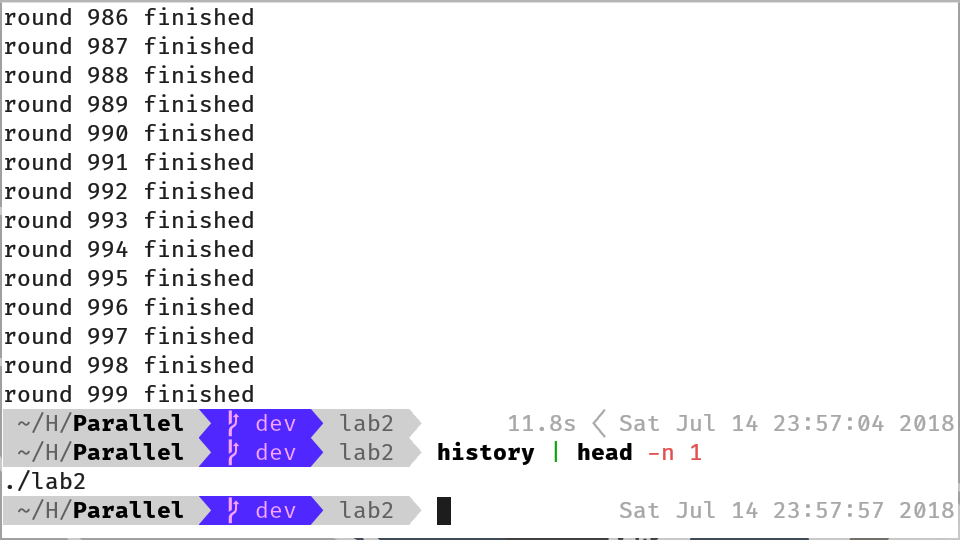
\includegraphics[width=0.9\linewidth]{pthreadOutput.png}
    \caption{pthread程序运行时间}
    \label{fig:pthreadOutput}
\end{figure}

\par 经过8组、每组3次的测试,加速比随线程变化的曲线如图\ref{fig:pthreadTrend}所示。可以看出,在线程数为1\textasciitilde 4时加速比随着线程数几乎呈线性变化,而在线程数为1时加速比为1.006,overhead所占用的时间几乎可以不计。在线程数达到4时由于物理内核已经被占满,因此后面加速比不再增加,随着线程数量的进一步增大,由于线程调度的开销,因此程序的加速比不再增加,反而有所下降。
\begin{figure}[htpb]
    \centering
    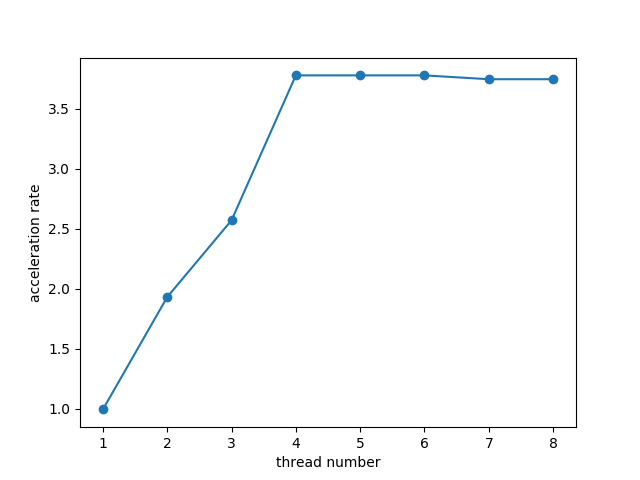
\includegraphics[width=0.8\linewidth]{pthreadTrend.png}
    \caption{加速比随线程数变化}
    \label{fig:pthreadTrend}
\end{figure}

\par 对于分块大小而言,加速比随着分块大小的变化如图\ref{fig:pthreadTrend2}所示,在分块大小较小时,加速比随着分块大小的变化并不大,只在分块大小过小时由于线程调度导致一点性能开销。当分块大小大于原图的一半时总时间则取决于分到最大分块线程所用的时间,因此在这个区间内性能随分块大小呈下降趋势。
\begin{figure}[htpb]
    \centering
    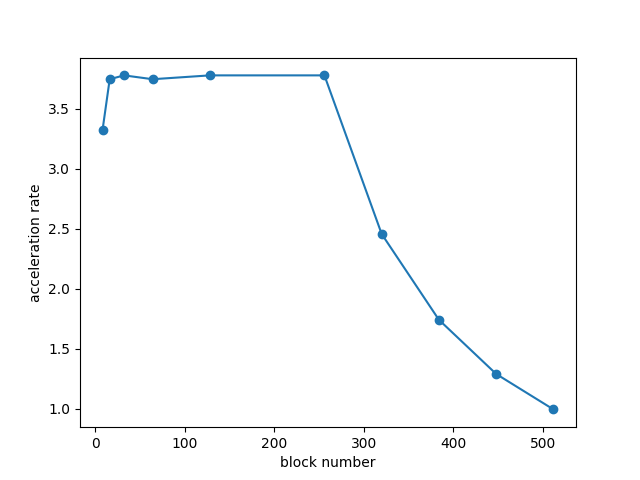
\includegraphics[width=0.8\linewidth]{pthreadTrend2.png}
    \caption{加速比随分块大小变化}
    \label{fig:pthreadTrend2}
\end{figure}




% chapter 3
\chapter{基于OpenMP的形态学图像处理}
\section{实验目的与要求}
\begin{enumerate}
    \item 掌握使用OpenMP进行并行编程设计和性能优化的基本原理和方法
    \item 使用OpenMP实现形态图像处理操作的并行算法
    \item 对程序执行结果进行简单的分析和总结
    \item 将其与Lab2的结果进行比较
\end{enumerate}

\section{算法描述}
\par 使用OpenMP进行并行计算与使用pthread进行并行计算的算法原理几乎一样,只不过OpenMP由编译器进行底层实现,使用for循环进行包装,且主线程不是空闲的,而是也参与计算。而pthread则需要人工进行底层的编写。使用OpenMP的关键部分代码如下:
\inputCodeSetLanguage{c++}
\begin{lstlisting}
#pragma omp parallel for num_threads(threadNum) schedule(dynamic, 2)
for(int i=0; i < workNum; ++i){
    // Code equvilent to calling ErodeAndDilate(blk, kernel_e, kernel_d)
}
\end{lstlisting}
\par OpenMP caluse中的schedule(dynamic, 2)将所有的人物按照2个一组进行分组,而每个线程领取一组任务、执行完成后在领取下一组可能的任务,从而避免了由于静态调度以及线程执行时间不等带来的CPU空闲。

\section{实验方案}
\par 由于算法与pthread基本相同,因此可以在pthread的实现上进行修改,将pthread中的线程竞争调度改为使用openmp directive包装的for循环,并在编译条件中去除-lpthread,加上-fopenmp即可。
\par 在运行时,通过多次调节参数并进行重复实验,得到一侧较优的参数,然后将这个参数与phtread实现进行对比,观察OpenMP实现与pthread实现的区别。

\section{实验结果与分析}
\par 功能上,OpenMP能够正确的处理图片并给出与串行处理相同的结果。性能上,使用4线程、分块大小128时程序的运行结果如图\ref{fig:ompOutput}所示。三次测试平均结果为12.63s,相对于串行程序加速比为\(44.2\div 12.63 = 3.49\),与同条件下的pthread实现比起来加速比要低不少,这是由于OpenMP需要进行环境的初始化,且其调度过程没有特别为底层实现的pthread程序优化,因此pthread实现的并行程序性能较为优秀。
\begin{figure}[htpb]
    \centering
    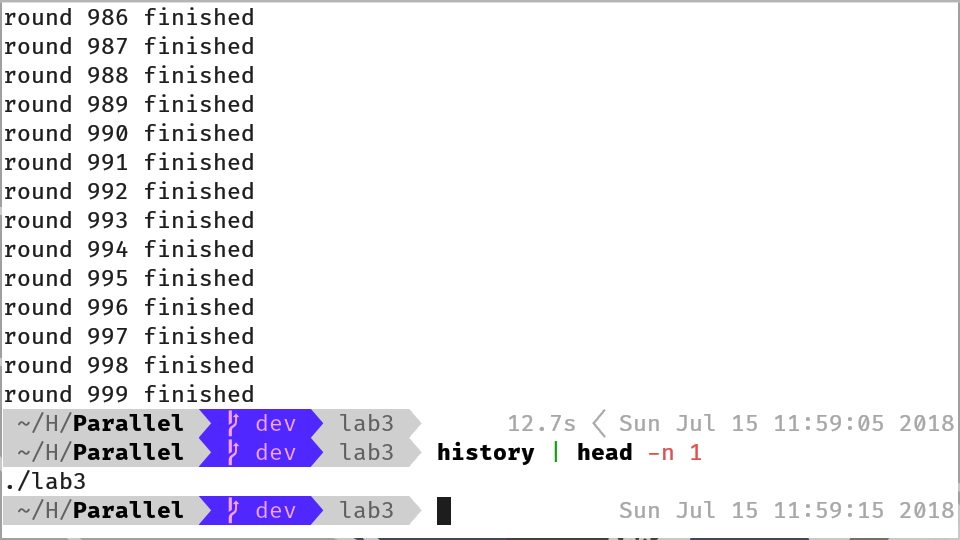
\includegraphics[width=0.9\linewidth]{ompOutput.png}
    \caption{使用OpenMP进行处理的输出}
    \label{fig:ompOutput}
\end{figure}

\par 加速比随线程数量变化如图\ref{fig:ompTrend}所示,其中实线部分为使用OpenMP的程序,而虚线部分为上述使用pthread的程序。从图中可以看出,使用OpenMP和使用pthread程序的性能随着线程数量的变化趋势是一样的,因为其算法本质上是相同的。而使用OpenMP的程序在同样的情况下总是比使用pthread的程序要慢一些,这也是由于OpenMP并不是一个针对特殊程序的调度算法,因此没有更为底层的,为特殊目的设计的pthread程序性能高,但在仅需要编写较少代码的情况下能够达到与pthread程序接近的性能说明其实现也是十分优秀的。
\begin{figure}[htpb]
    \centering
    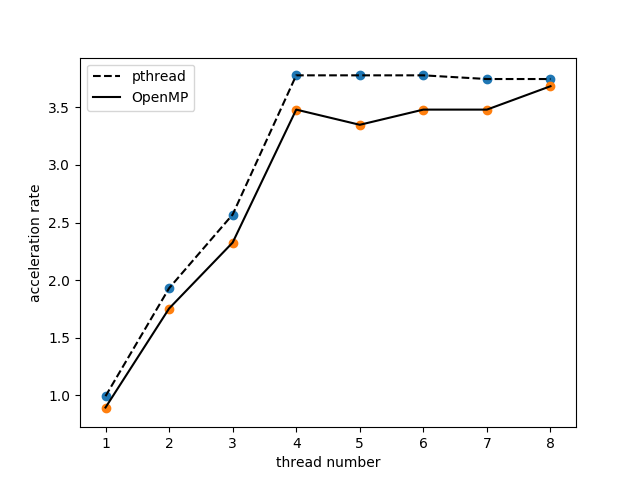
\includegraphics[width=0.8\linewidth]{ompTrend.png}
    \caption{加速比随线程数量变化}
    \label{fig:ompTrend}
\end{figure}
\par 而加速比随分块大小的变化如图\ref{fig:ompTrend2}所示,同样,实线为OpenMP实现,虚线为pthread实现。与随着线程变化的趋势一样,在同样的情况下OpenMP的性能比pthread性能低。在分块大小超过图片的1/2时更为明显,其下降趋势更为剧烈,推测是由于OpenMP的启动与初始化时间以及调度的分块引起的。
\par 从上述结果可以得出结论:在对于并行性能要求不是非常高时,使用OpenMP可以简化程序编写者的工作量,而使用pthread作出针对特定程序的并行算法则相对于OpenMP算法可以较大的提高程序的性能。
\begin{figure}[htpb]
    \centering
    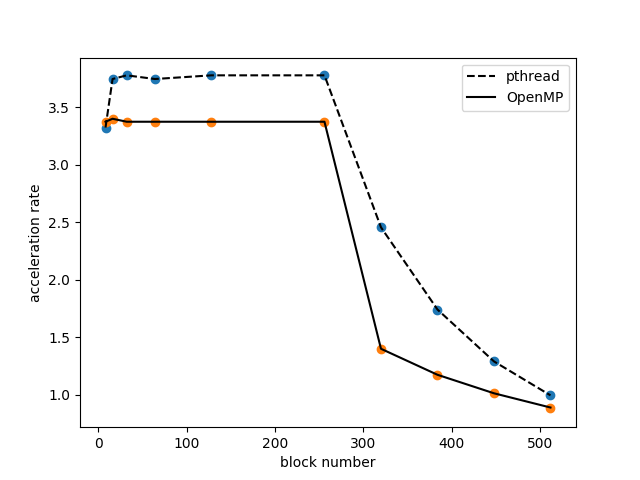
\includegraphics[width=0.8\linewidth]{ompTrend2.png}
    \caption{加速比随线分块大小变化}
    \label{fig:ompTrend2}
\end{figure}




% chapter 4

\chapter{基于MPI的形态学图像处理}
\section{实验目的与要求}
\begin{enumerate}
    \item 掌握使用MPI进行并行编程设计和性能优化的基本原理和方法
    \item 使用MPI实现形态图像处理操作的并行算法
    \item 对程序执行结果进行简单的分析和总结
    \item 将其与Lab2和Lab3的结果进行比较
\end{enumerate}

\section{算法描述}
\par 对于MPI而言,由于其编程框架与OpenMP是不同的,因此需要使用不同的方法。由于在计算蚀刻以及膨胀时要使用一个像素周围的所有像素,如图\ref{fig:overlap}所示,因此如果使用\lstinline{MPI_Scatter}进行数据的分散则需要考虑分块边缘重叠的部分,实际上加大了程序编写的复杂度,而OpenMP和pthread程序由于是基于内存共享模型的因此不存在这一问题。而且由于需要对于重叠的部分进行额外的复制,若使用Scatter进行分散因此实际上降低了程序的性能。出于以上的考虑,直接使用Bcast将整张图片进行广播。

\begin{figure}[htpb]
    \centering
    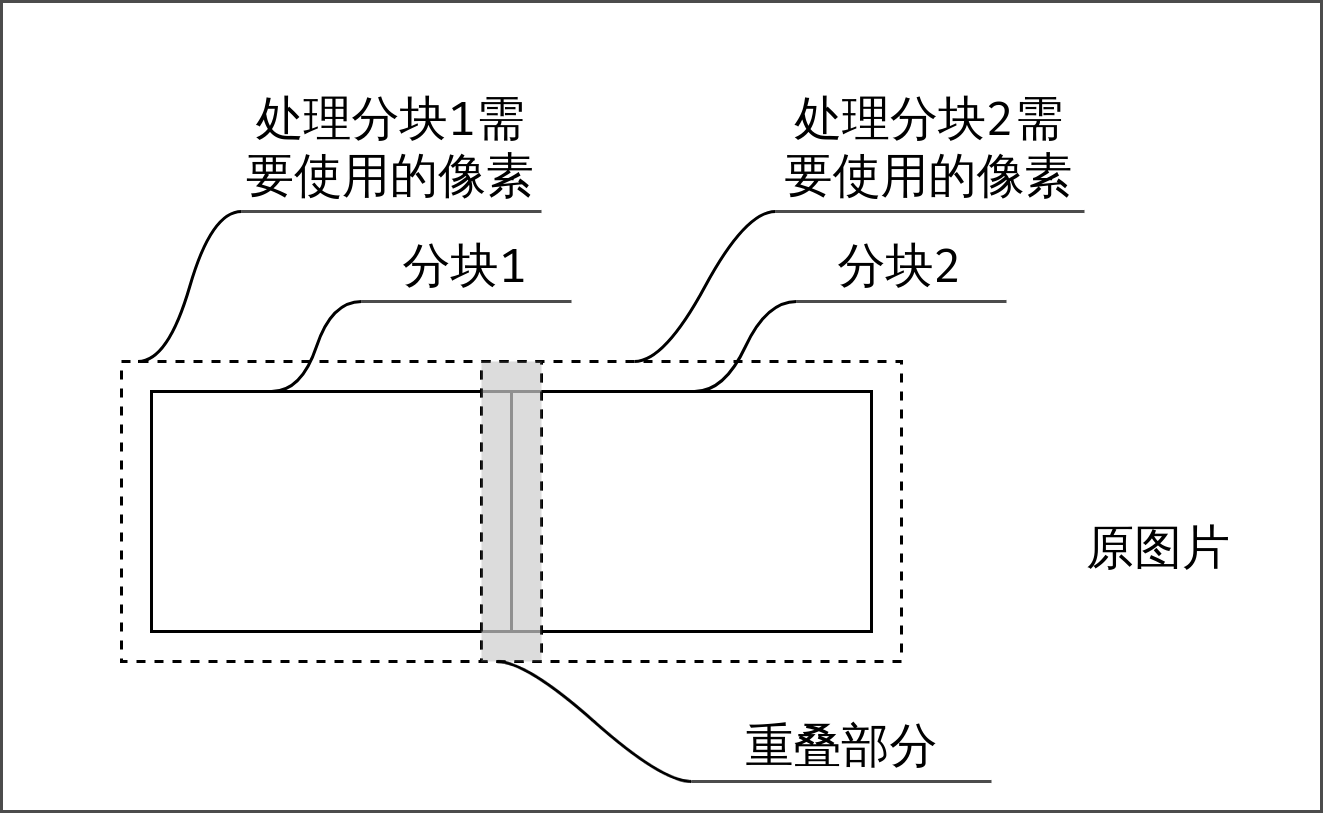
\includegraphics[width=0.6\linewidth]{overlap.png}
    \caption{两个分块的重叠部分}
    \label{fig:overlap}
\end{figure}

\par 将整张图片进行广播后,每个进程根据总的进程数量处理自己的分块,而新的分块方式如图\ref{fig:partition2}所示,在原图片的y方向上进行分块,除了主进程外每一个进程取与自己的编号相同的分块进行处理,最后使用\lstinline{MPI_Gather}对于处理的部分进行回收与拼接。由于在广播阶段广播整张图片,因此在处理时不需要考虑边缘重叠问题,此外,考虑到进程间数据传递的效率较线程间数据传递的效率低,因此不使用一个进程处理多个分块的方式,而是直接处理一个较大的分块直到处理完成。由于各个进程处理的数据量几乎一致,且处理逻辑是同质的,因此预计各个进程的处理时间不会相差太多。
\begin{figure}[htpb]
    \centering
    
\includegraphics[width=0.5\linewidth]{partition2.png}
    \caption{新的分块方式}
    \label{fig:partition2}
\end{figure}
\par 与pthread类似,在使用MPI进行并行处理时需要有一个主线程等待其他所有线程的完成,起到调度的作用。

\section{实验方案}
\par 依据实验思路进行代码的编写后编译进行测试。需要注意的是编译需要使用OpenMPI的包装编译器mpic++进行编译,在运行时也需要使用mpirun运行。多次改变进程数量后与前两次实验进行对比。

\section{实验结果与分析}
\par 使用4进程运行的结果如图\ref{fig:mpiOutput}所示,此输出在4个线程下运行得到。可以看到,程序运行时间为15.9s,相对于串行的加速比为\(44.2\div 15.9 = 2.77\),由于主线程不参与计算,因此这一结果与理想加速比3是比较接近的。
\par 对于其他进程数而言,由于有一个主进程,因此至少需要两个进程才能完整运行程序,而由于进程数不能超过物理内核数,因此实际测试的进程数只有2、3、4这3种情况,除掉主进程,有效进程数分别为1、2、3,与pthread和OpenMP进行对比的结果如图\ref{fig:mpiTrend}所示。可以看到其与pthread的性能相差无几。

\begin{figure}[htpb]
    \centering
    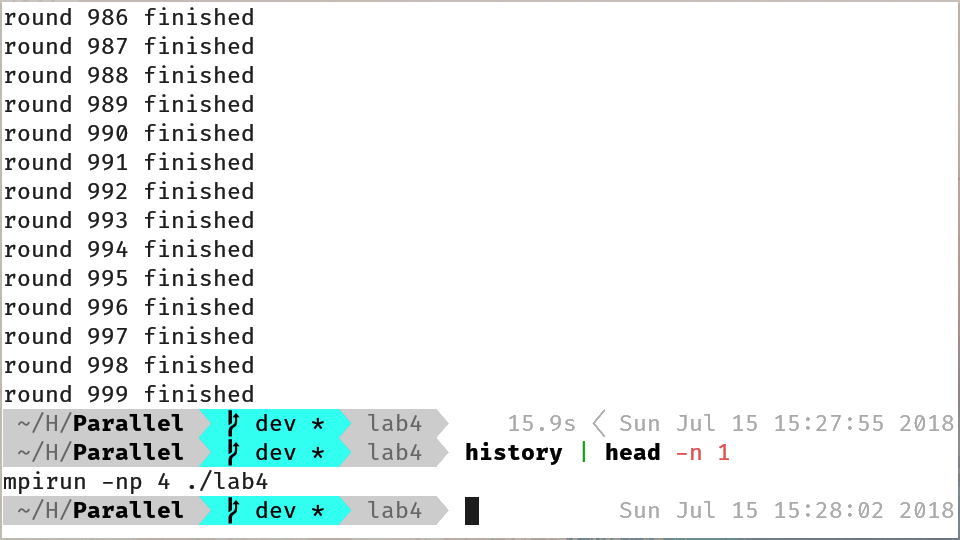
\includegraphics[width=0.8\linewidth]{mpiOutput.png}
    \caption{MPI程序输出}
    \label{fig:mpiOutput}
\end{figure}

\begin{figure}[htpb]
    \centering
    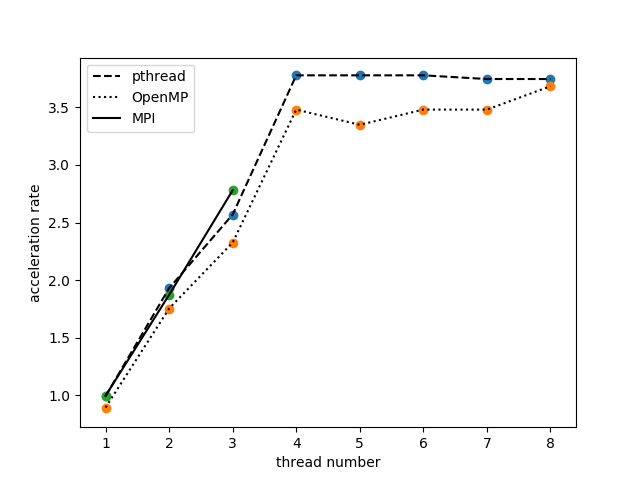
\includegraphics[width=0.8\linewidth]{mpiTrend}
    \caption{MPI程序与OpenMP、pthread程序的对比结果}
    \label{fig:mpiTrend}
\end{figure}




% chapter 5
\chapter{基于CUDA的形态学图像处理}
\section{实验目的与要求}
\begin{enumerate}
    \item 深入理解GPGPU的架构并掌握CUDA编程模型
    \item 使用CUDA实现形态图像处理操作的并行算法
    \item 对程序执行结果进行简单的分析和总结
    \item 根据执行结果和硬件环境提出优化解决方案
    \item 将其与Lab2,Lab3和Lab4的结果进行比较
\end{enumerate}

\section{算法描述}
\par 与上述并行算法不同的是,CUDA使用的是异构的并行算法,由于GPU本身就比较适合进行图像处理,因此预计相对于串行算法的加速比会比较高。同样,按照pthread实验中的方法对于图片进行分块,然后将每一个图片块分配给不同的CUDA block,将块中的不同像素分配给不同的CUDA Thread进行处理。如图\ref{fig:cudaScheme}所示,线程的处理过程与算法ErodeAndDilate相同。
\begin{figure}[htpb]
    \centering
    
\includegraphics[width=0.4\linewidth]{cudaScheme.png}
    \caption{CUDA块与线程分配}
    \label{fig:cudaScheme}
\end{figure}

\section{实验方案}
\par 编写CUDA程序并进行测试,在编译时需要使用CUDA的包装编译器nvcc进行编译,,在运行时需要保证Nvidia驱动已被正确加载。

\section{实验结果与分析}
\par 图像处理的结果与串行图像处理的结果相同,性能方面,程序在使用分块大小为128,每个像素使用一个线程处理的情况下,处理时间如图\ref{fig:cudaOutput}所示,可以看出,程序只使用了989ms就完成了1000次处理,相对与并行程序加速比达到了44.7,由此可见CUDA是较为适合并行处理图片的。

\begin{figure}[htpb]
    \centering
    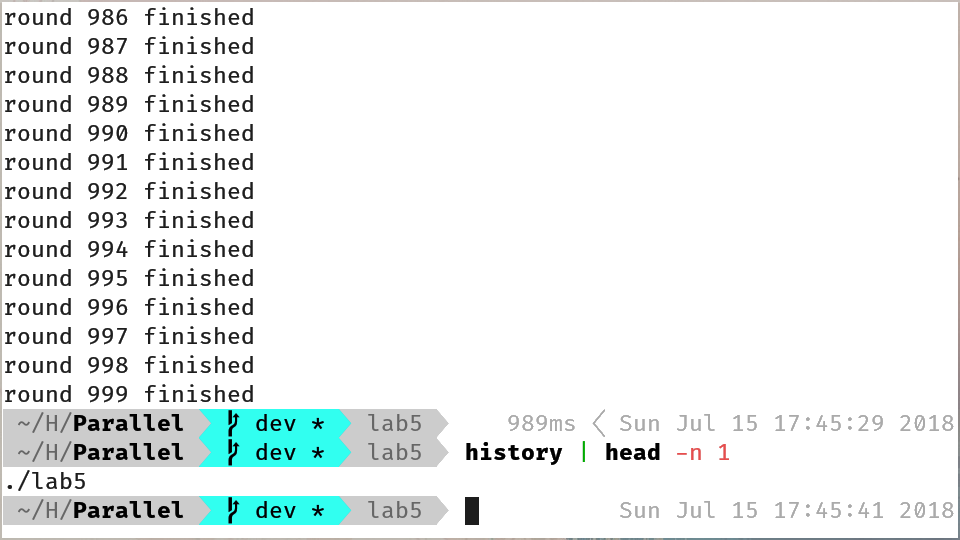
\includegraphics[width=0.9\linewidth]{cudaOutput.png}
    \caption{CUDA程序运行结果}
    \label{fig:cudaOutput}
\end{figure}
\par 由于CUDA架构与仅使用CPU并行的架构完全因此不同,因此不具备与CPU程序在性能上的可比性。在不同的块大小情况下,CUDA程序的最优时间为686ms,相对于串行程序的加速比达到了64.31,由此可见,对于数据易于分块,数据间无依赖的简单数据使用GPU进行处理占有绝对优势。


\chapter{基于并行回溯算法的数独求解算法}
\section{实验目的与要求}
\begin{enumerate}
    \item 掌握并行化和改进程序的方法
    \item 了解并行粒度与性能之间的关系
    \item 掌握如何分割数据和分解复杂算法的任务
\end{enumerate}

\section{算法描述}
\par 数独的规则见\url{https://zh.wikipedia.org/zh-sg/%E6%95%B8%E7%8D%A8}。一个未求解和已经进行求解的数独如图\ref{fig:unsolved}和\ref{fig:solved}所示。
\begin{figure}[htpb]
    \centering
    \begin{minipage}{0.45\linewidth}
        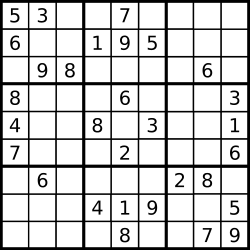
\includegraphics[width=0.9\linewidth]{unsolved.png}
        \caption{未求解的数独}
        \label{fig:solved}
    \end{minipage}
    \hfill
    \begin{minipage}{0.45\linewidth}
        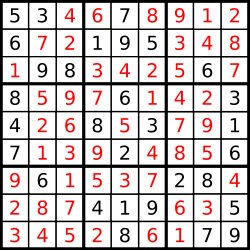
\includegraphics[width=0.9\linewidth]{solved.png}
        \caption{已经求解的数独}
        \label{fig:unsolved}
    \end{minipage}
\end{figure}
\par 首先,需要一个串行的数独求解程序进行参考,串行的程序使用回溯的方法对于数独进行求解,同样,为了便于时间的统计,因此需要增加求解的数据量,此时,对于100个数独进行求解。
\par 然后需要设计一个并行的数独求解程序。由于数独前后的逻辑依赖性较强,因此不便于进行并行。在本实验中采用的数独求解方法为并行化的测试一个cell中的所有case,以求获得最小的可能的case的时间。此时,case的选择可以在不同的遍历层级进行。递归的层级越高则粒度越低。

\section{实验方案}
\par 按照算法描述中的算法编写OpenMP程序,在小于特定层级时将所有的可能性如队列,然后在这一特定的层级使用OpenMP进行并行,在大于这一层级不再使用并行算法,以避免线程数量指数爆炸。
\par 需要注意的是在一个线程找到结果后需要及时停止其他的线程,而在停止时不可以使用C++ exception,经过性能测试,exception带来的开销约为20\%,极大的开销会为程序带来负优化。线程的错误处理一定因此通过返回值的方式进行。

\section{实验结果与分析}
\par 串行程序解决100个数独的结果如图\ref{fig:sudoSerial}所示。数独题目由qqwing程序生成,所有答案经过验证均正确。从图中可以看出,串行的程序需要使用25.8s进行求解。
\begin{figure}[htpb]
    \centering
    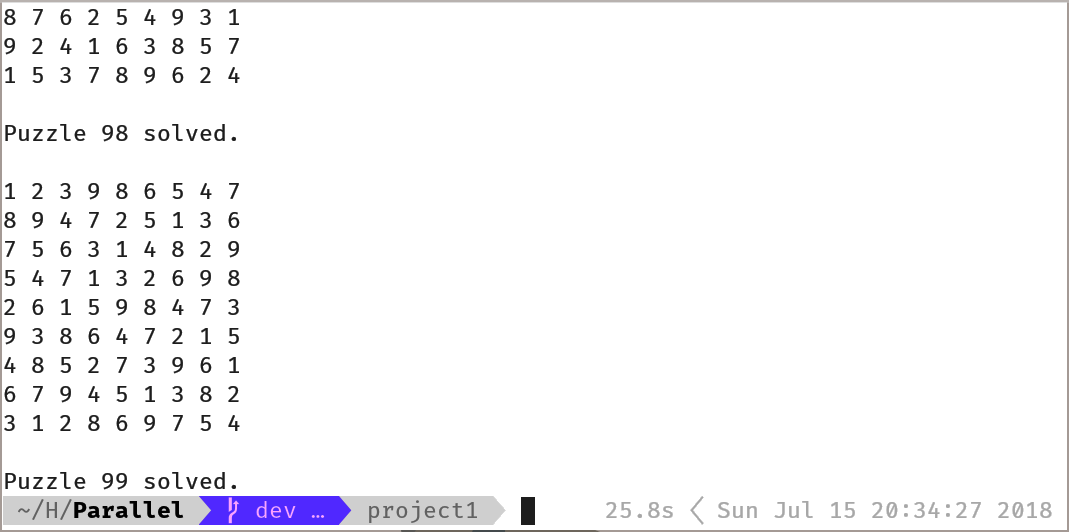
\includegraphics[width=0.9\linewidth]{sudoSerial.png}
    \caption{串行数独求解}
    \label{fig:sudoSerial}
\end{figure}
\par 在递归的第二层进行4线程并行的时间如图\ref{fig:sudoParallel}所示,从图中可以看出,需要2.96s进行求解,相比于串行程序,加速比为8.71,达到了较为理想的加速比。

\begin{figure}[htbp]
    \centering
    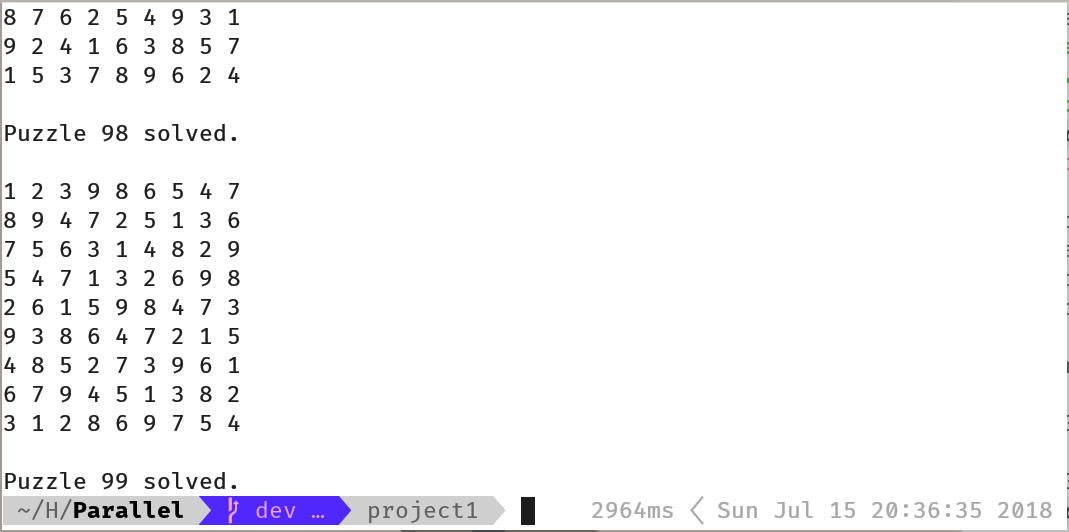
\includegraphics[width=0.9\linewidth]{sudoParallel.png}
    \caption{4线程并行数独求解}
    \label{fig:sudoParallel}
\end{figure}
\par 加速比与粒度的关系如图\ref{fig:sudoTrend}所示。可以看出,粒度越细加速比越低,这是由于前边的并行部分增大以及线程竞争引起的。

\begin{figure}[htbp]
    \centering
    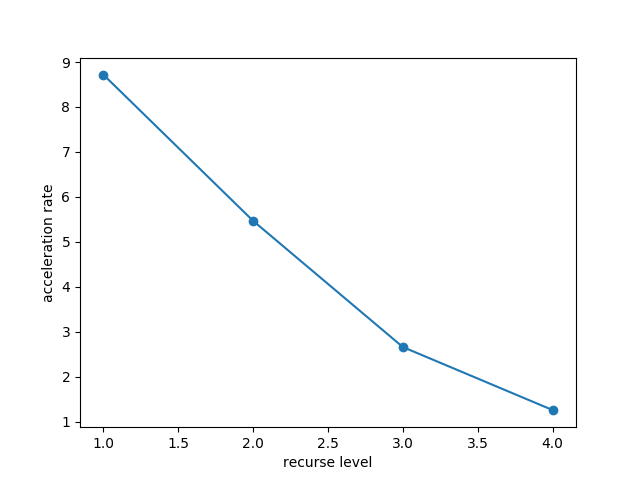
\includegraphics[width=0.8\linewidth]{sudoTrend.png}
    \caption{加速比随粒度的变化关系}
    \label{fig:sudoTrend}
\end{figure}

\appendix
\chapter{开发与运行环境}
\label{cha:env}

\par 所有lab的开发与运行的环境的平台、版本如表\ref{tab:env}所示。
\begin{table}[htpb]
    \centering
    \caption{开发与运行环境}
    \label{tab:env}
    \begin{tabular}{ c r l }
        \toprule
        \multicolumn{1}{c}{} &
        \multicolumn{1}{c}{项目} &
        \multicolumn{1}{c}{版本} \\
        \cmidrule(lr){1-1} \cmidrule(lr){2-2} \cmidrule(lr){3-3}
        \multirow{8}{*}{软件} & 操作系统    & ArchLinux,  Kernel version 4.17.5-1\\
                              & gcc             & 8.1.1     \\
                              & GNU Make        & 4.2.1     \\
                              & OpenMP          & 6.0.1     \\
                              & OpenMPI         & 3.1.0-1   \\
                              & CUDA            & 9.2.148-1 \\
                              & Nvidia driver   & 396.24-15 \\
                              & shell           & fish 2.7.1\\
        \cmidrule(lr){1-1} \cmidrule(lr){2-2} \cmidrule(lr){3-3}
        \multirow{3}{*}{硬件} & CPU             & Intel Core i7-7700K CPU @ 4.20GHz \\
                              & GPU             & NVIDIA Corporation GP102 [GeForce GTX 1080 Ti] \\
                              & RAM             & Kingston DDR4 16GiB (\(\times 2\))\\
        \bottomrule
    \end{tabular}
\end{table}

\par 目录结构如下
\inputCodeSetLanguage{bash}
\begin{lstlisting}
./                          project根目录
├── README.md               README文件(本文件)
├── Makefile                主Makefile,用于同时编译/清除所有lab
├── data                    数据目录
│   ├── Lenna.png           lab1 ~ lab5 所用图片
│   └── questions.txt       lab6 所用数独数据
├── lab1                    串行形态学图像处理
│   ├── Makefile            lab1 Makefile
│   └── main.cpp            lab1 源码
├── lab2                    使用pthread加速的多线程图像处理
│   ├── Makefile            lab2 Makefile
│   └── main.cpp            lab2 源码
├── lab3                    使用openmp加速的多线程图像处理
│   ├── Makefile            lab3 Makefile
│   └── main.cpp            lab3 源码
├── lab4                    使用openmpi加速的多线程图像处理
│   ├── Makefile            lab4 Makefile
│   ├── main.cpp            lab4 源码
│   └── run.sh              openmpi 运行环境的包装,使用mpirun执行编译输出
├── lab5                    使用cuda加速的多线程图像处理
│   ├── Makefile            lab5 Makefile
│   └── main.cu             lab5 源码
├── project1                数独求解程序
│   ├── Makefile            lab6 Makefile
│   ├── parallel.cpp        使用openmp加速的并行数独求解程序源码
│   └── serial.cpp          串行数独求解程序源码
├── lib                     第三方库文件夹
│   └── CImg-2.3.3          CImg图像处理库
│       └── ...             CImg图像处理库内容
└── report                  报告文件夹
        └── ...             报告内容
\end{lstlisting}

\par 要正常的编译和运行,需要保证gcc、nvcc所在的目录在\$PATH中。

\par 要能够正确的编译并运行lab5,需要满足下列要求:
\begin{itemize}
    \item nvcc在\$PATH中
    \item PC上装有支持cuda的Nvidia显卡
    \item 正确版本的Nvidia驱动以正确安装并 **已加载**
    \item Nvidia显卡有足够的显存以及足够的Concurrent Thread数目以支持程序的运行。
\end{itemize}

\par 此外,lab2、lab3可以使用`-n <number>`来指定线程数,使用`-s <number>` 来指定图片分块大小 (推荐在8~256之间) ;lab4可以通过更改`run.sh`更改进程数,进程数必须大于1,但不可超过CPU物理内核数。


\vfill
{\tiny written by HuSixu \hfill powered by \XeLaTeX .}

\end{document}
